\documentclass[border=6pt]{standalone}
\usepackage{amsmath,amssymb}
\usepackage{tikz}
\usetikzlibrary{arrows.meta,calc,decorations.pathreplacing,patterns,shapes.geometric,positioning,shadings,plotmarks}

\begin{document}
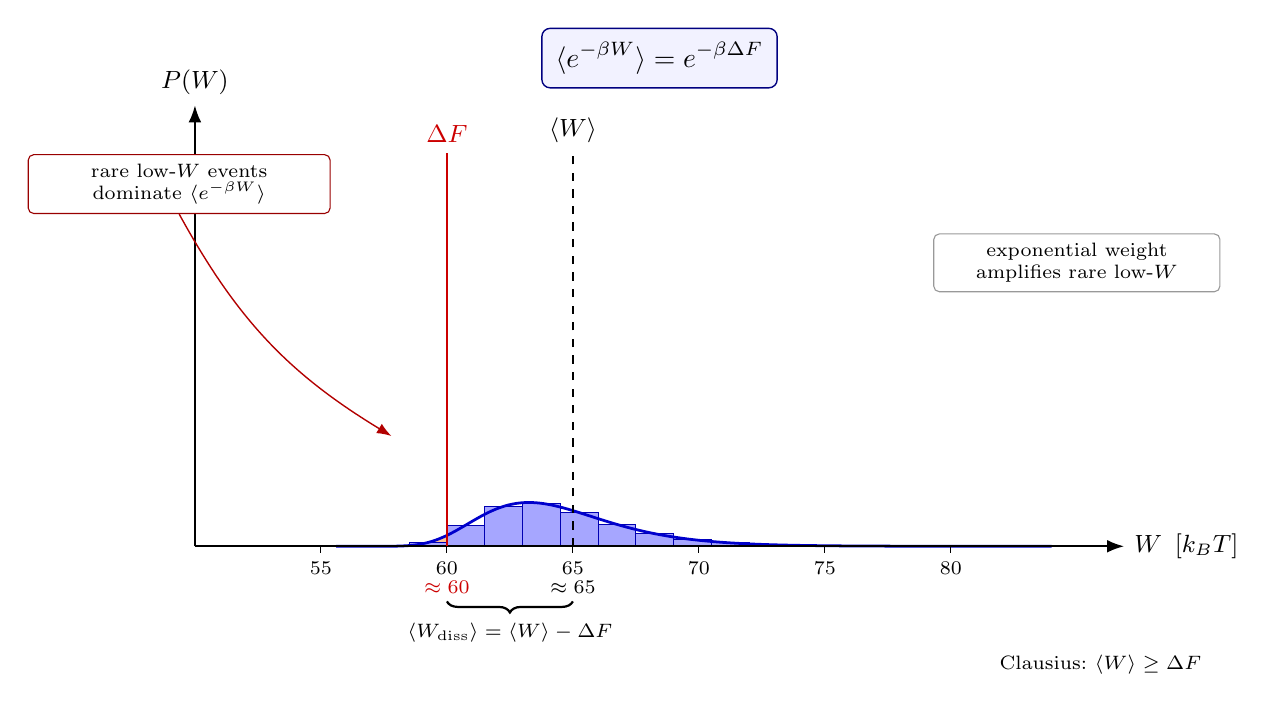
\begin{tikzpicture}[>=Latex,scale=1.0,every node/.style={font=\small}]

% ============================================================
% Axes
% ============================================================
% W axis: from W=50 to W=85 (k_B T units), peak around W ~ 64
% P axis: 0 to ~0.42
\def\Wmin{50}
\def\Wmax{85}
\def\Wscale{0.32} % cm per kBT
\def\Pscale{12}   % cm per probability unit (max ~0.42 -> ~5cm)

% Origin and axes coordinates
\coordinate (O) at (0,0);
\coordinate (XEnd) at ({(\Wmax-\Wmin)*\Wscale + 0.6},0);
\coordinate (YEnd) at (0,5.6);

% ============================================================
% Lognormal-like distribution: P(W) ~ exp(-(W-mu)^2/(2 s^2)) with right skew
% Use a skewed bell. We'll define a function approximating right-skew lognormal:
% f(W) = A * exp( -((ln(W-W0) - m)^2)/(2 s^2) ) / (W - W0)
% Choose W0 = 55 (shift), m = ln(9) ~ 2.20, s = 0.30
% Peak at exp(m - s^2) + W0 ~ exp(2.11) + 55 ~ 8.25 + 55 = 63.25
% mean ~ exp(m + s^2/2) + W0 ~ exp(2.245) + 55 ~ 9.44 + 55 = 64.44 (~ <W>=65)
% ============================================================

% Histogram bars (discrete bins of width 1.5 kBT)
\def\W0{55}

% Helper: declare the distribution coordinates for fill region
% We'll use \pgfmathparse to compute heights at sample bin centers.

% Shaded left tail region (for W < Delta F = 60)
% Fill under curve from W=55.5 to W=60 with red-orange gradient
\begin{scope}
  \clip ({(55.5-\Wmin)*\Wscale},0)
    -- plot[domain=55.5:60, samples=40, smooth]
       ({(\x-\Wmin)*\Wscale},
        {\Pscale * 0.40 * exp(-((ln(\x-\W0) - 2.20)^2)/(2*0.09)) / (\x-\W0)})
    -- ({(60-\Wmin)*\Wscale},0) -- cycle;
  \shade[left color=red!55,right color=orange!50,opacity=0.85]
    ({(55.5-\Wmin)*\Wscale},0) rectangle ({(60-\Wmin)*\Wscale},5.5);
\end{scope}

% Histogram (blue bars), bin width 1.5
\foreach \binc in {56.25,57.75,59.25,60.75,62.25,63.75,65.25,66.75,68.25,69.75,71.25,72.75,74.25,75.75,77.25,78.75,80.25,81.75,83.25}
{
  \pgfmathsetmacro{\hgt}{\Pscale * 0.40 * exp(-((ln(\binc-\W0) - 2.20)^2)/(2*0.09)) / (\binc-\W0)}
  \pgfmathsetmacro{\xL}{(\binc - 0.75 - \Wmin)*\Wscale}
  \pgfmathsetmacro{\xR}{(\binc + 0.75 - \Wmin)*\Wscale}
  \ifdim \hgt pt > 0.02pt
    \draw[fill=blue!35,draw=blue!70!black,line width=0.3pt]
      (\xL,0) rectangle (\xR,\hgt);
  \fi
}

% Smooth distribution curve overlay
\draw[blue!80!black,line width=1.0pt,smooth,samples=80,domain=55.6:84]
  plot ({(\x-\Wmin)*\Wscale},
    {\Pscale * 0.40 * exp(-((ln(\x-\W0) - 2.20)^2)/(2*0.09)) / (\x-\W0)});

% ============================================================
% Axes drawn on top of histogram
% ============================================================
\draw[->,line width=0.7pt] (O) -- (XEnd) node[right]{$W\ \,[k_B T]$};
\draw[->,line width=0.7pt] (O) -- (YEnd) node[above]{$P(W)$};

% X-axis ticks
\foreach \w in {55,60,65,70,75,80}
{
  \pgfmathsetmacro{\xpos}{(\w - \Wmin)*\Wscale}
  \draw (\xpos,0) -- (\xpos,-0.08) node[below,font=\scriptsize]{\w};
}

% ============================================================
% Vertical markers: Delta F (red, solid) and <W> (black, dashed)
% ============================================================
\pgfmathsetmacro{\xDF}{(60 - \Wmin)*\Wscale}
\pgfmathsetmacro{\xWa}{(65 - \Wmin)*\Wscale}

% Delta F line (red solid)
\draw[red!80!black,line width=1.0pt] (\xDF,0) -- (\xDF,5.0);
\node[red!80!black,above,font=\small] at (\xDF,5.0) {$\Delta F$};
\node[red!80!black,below=2pt,font=\scriptsize] at (\xDF,-0.25) {$\approx 60$};

% <W> line (black dashed)
\draw[black,dashed,line width=0.9pt] (\xWa,0) -- (\xWa,5.0);
\node[above,font=\small] at (\xWa,5.0) {$\langle W\rangle$};
\node[below=2pt,font=\scriptsize] at (\xWa,-0.25) {$\approx 65$};

% Brace between Delta F and <W>: <W_diss>
\draw[decorate,decoration={brace,amplitude=4pt,mirror},thick]
  (\xDF,-0.7) -- (\xWa,-0.7)
  node[midway,below=4pt,font=\scriptsize]{$\langle W_{\rm diss}\rangle = \langle W\rangle - \Delta F$};

% ============================================================
% Annotation for rare low-W tail
% ============================================================
\coordinate (TailMid) at ({(57.8-\Wmin)*\Wscale},1.4);
\coordinate (TailLabel) at (-0.2,4.6);
\node[draw=red!60!black,fill=white,rounded corners=2pt,
      align=center,font=\scriptsize,line width=0.4pt,
      text width=3.6cm] (TL) at (TailLabel)
  {rare low-$W$ events\\ dominate $\langle e^{-\beta W}\rangle$};
\draw[->,red!70!black,line width=0.5pt] (TL.south) to[bend right=15] (TailMid);

% Right-side annotation
\node[draw=black!40,fill=white,rounded corners=2pt,
      align=center,font=\scriptsize,text width=3.4cm,line width=0.4pt]
  at ({(\Wmax-\Wmin)*\Wscale - 0.0},3.6)
  {exponential weight\\ amplifies rare low-$W$};

% ============================================================
% Top equation
% ============================================================
\node[draw=blue!50!black,fill=blue!5,rounded corners=3pt,
      line width=0.5pt,font=\normalsize,inner sep=5pt]
  at ({((\Wmax-\Wmin)*\Wscale)/2 + 0.3}, 6.2)
  {$\displaystyle \langle e^{-\beta W}\rangle = e^{-\beta \Delta F}$};

% Bottom-right inequality annotation
\node[font=\scriptsize,align=right]
  at ({(\Wmax-\Wmin)*\Wscale + 0.3}, -1.5)
  {Clausius:\ $\langle W\rangle \ge \Delta F$};

\end{tikzpicture}
\end{document}
